\documentclass{beamer}
\usefonttheme[onlymath]{serif}

% Code Block Setting
\usepackage{listings}
\lstset{language=C,
numberstyle=\footnotesize,
basicstyle=\ttfamily\footnotesize,
numbers=left,
stepnumber=1,
frame=shadowbox,
breaklines=true}

\usetheme{Warsaw}
% \usecolortheme{dove}

% Add frame number and total frame number in footline
\defbeamertemplate*{footline}{shadow theme}{%
    \leavevmode%
    \hbox{\begin{beamercolorbox}[wd=.5\paperwidth,ht=2.5ex,dp=1.125ex,leftskip=.3cm plus1fil,rightskip=.3cm]{author in head/foot}%
            \usebeamerfont{author in head/foot}\hfill\insertshortauthor
        \end{beamercolorbox}%
        \begin{beamercolorbox}[wd=.4\paperwidth,ht=2.5ex,dp=1.125ex,leftskip=.3cm,rightskip=.3cm plus1fil]{title in head/foot}%
            \usebeamerfont{title in head/foot}\insertshorttitle\hfill%
        \end{beamercolorbox}%
        \begin{beamercolorbox}[wd=.1\paperwidth,ht=2.5ex,dp=1.125ex,leftskip=.3cm,rightskip=.3cm plus1fil]{title in head/foot}%
            \hfill\insertframenumber\,/\,\inserttotalframenumber
    \end{beamercolorbox}}%
    \vskip0pt%
}

% Tikz related
\usepackage{tikz}
\usetikzlibrary{fit}
\usetikzlibrary{calc}
\usetikzlibrary{positioning}

% Number the figures
\setbeamertemplate{caption}[numbered]

% Add outline page at begining of each section
\AtBeginSection[]
{
    \begin{frame}<beamer>
        \frametitle{Outline}
        \tableofcontents[currentsection, hideallsubsections]
    \end{frame}
}

%%%%%%%%%%%%%%%%%%%%%%%%%%%%%%%%%%%%%%%%%%%%%

\title{yaSpMV: Yet Another SpMV Framework on GPUs}
\author{
    Shengen Yan\inst{1}\\
    Chao Li \inst{1}\\
    Yunquan Zhang\inst{2}\\
    Huiyang Zhou \inst{1}
}
\institute{
    \inst{1} North Carolina State Universit\\
    \inst{2} Chinese Academy of Sciences Institute of Software
}
\date{
    \tiny{Principles and Practice of Parallel Programming 2014}\\
    \tiny{Presented by ShiangYun Yang}
}

\begin{document}
\begin{frame}
    \titlepage
\end{frame}

\section{Introduction}

\subsection{SIMD}
\begin{frame}
    \frametitle{SIMD}
	\begin{itemize}
		\item Single instruction multiple data
		\item without threads support
	\end{itemize}
\end{frame}


\subsection{VPU}
\begin{frame}
    \frametitle{VPU}
	\begin{itemize}
		\item Vector processing units 
		\item combine itstructions as vector	
	    \begin{figure}
			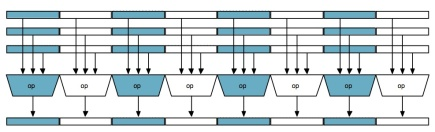
\includegraphics[scale=0.5]{figure/vpu.jpg}
		\end{figure}
	\end{itemize}
\end{frame}


\section{Matrix Data Format}

\subsection{COO Format}
\begin{frame}
    \frametitle{Common Coordinate Format (COO Format)}
	\begin{align*}
		A = \begin{bmatrix}
			0 & 0 & a & 0 & 0 & 0 & b & c \\
			0 & 0 & d & e & 0 & 0 & f & 0 \\
			0 & 0 & 0 & 0 & g & h & i & j \\
			k & l & 0 & 0 & m & n & o & p \\
		\end{bmatrix}
	\end{align*}
	\begin{align*}
		\text{Row index} &= [0, 0, 0, 1, 1, 1, 2, 2, 2, 2, 3, 3, 3, 3, 3, 3] \\
		\text{Col index} &= [2, 6, 7, 2, 3, 6, 4, 5, 6, 7, 0, 1, 4, 5, 6, 7] \\
		\text{Value}     &= [a, b, c, d, e, f, g, h, i, j, k, l, m, n, o, p]
	\end{align*}
	\begin{itemize}
		\item
    		COO Format has explicit storage for the column and row indices.
	\end{itemize}
\end{frame}

\subsection{BCOO Format}
\begin{frame}
	\frametitle{Block Common Coorindate Format (BCOO Format)}
	\begin{itemize}
		\item Block Common Coorindate Format extends the COO Format.
		\item First, using block size of $2 \times 2$ blocked COO format has 
			shown in figure.
	\end{itemize}
	\tikzset{%
  highlight/.style={rectangle,rounded corners,fill=red!15,draw,fill opacity=0.2,thick,inner sep=0pt}
}
\newcommand{\tikzmark}[2]{\tikz[overlay,remember picture,baseline=(#1.base)] \node (#1) {#2};}
%
\newcommand{\Highlight}[1][submatrix]{%
    \tikz[overlay,remember picture]{
      \node[highlight,fit=(left1.north west) (right1.south east)] (#1) {};
      \node[highlight,fit=(left2.north west) (right2.south east)] (#1) {};
    }
}


\begin{align*}
  A = \begin{bmatrix}
      0 & 0 & \tikzmark{left1}{a} & 0 & 0 & 0 & \tikzmark{left2}{b} & c \\
      0 & 0 & d & \tikzmark{right1}{e} & 0 & 0 & f & \tikzmark{right2}{0} \\
      0 & 0 & 0 & 0 & g & h & i & j \\
      k & l & 0 & 0 & m & n & o & p \\
    \end{bmatrix}
    \Highlight[first]
\end{align*}



\end{frame}

\subsection{BCCOO Format}
\begin{frame}
	\frametitle{From BCOO Format to BCCOO Format}
		Block Compressed Common Coordinate Format
		\begin{itemize}
			\item It uses difference function to compress row index array, and
				we get row index compression ratio equal $1/32$.
			\item If a difference value larger than 1, replace it with multiple 1s.
		\end{itemize}
\end{frame}

\begin{frame}
	\frametitle{BCCOO Format Example}
	\tikzset{%
  highlight/.style={rectangle,rounded corners,fill=red!15,draw,fill opacity=0.2,thick,inner sep=0pt}
}
\newcommand{\tikzmark}[2]{\tikz[overlay,remember picture,baseline=(#1.base)] \node (#1) {#2};}
%
\newcommand{\Highlight}[1][submatrix]{%
    \tikz[overlay,remember picture]{
      \node[highlight,fit=(left1.north west) (right1.south east)] (#1) {};
      \node[highlight,fit=(left2.north west) (right2.south east)] (#1) {};
    }
}


\begin{align*}
  A = \begin{bmatrix}
      0 & 0 & \tikzmark{left1}{a} & 0 & 0 & 0 & \tikzmark{left2}{b} & c \\
      0 & 0 & d & \tikzmark{right1}{e} & 0 & 0 & f & \tikzmark{right2}{0} \\
      0 & 0 & 0 & 0 & g & h & i & j \\
      k & l & 0 & 0 & m & n & o & p \\
    \end{bmatrix}
    \Highlight[first]
\end{align*}



\begin{align*}
	\text{Value} &= \left \{ \begin{bmatrix}
	a & 0\\ 
	d & e
	\end{bmatrix}, 
	\begin{bmatrix}
	b & c\\ 
	f & 0
	\end{bmatrix}, 
	\begin{bmatrix}
	0 & 0\\ 
	k & l
	\end{bmatrix}, 
	\begin{bmatrix}
	g & h\\ 
	m & n
	\end{bmatrix}, 
	\begin{bmatrix}
	i & j\\ 
	o & p
	\end{bmatrix}
	\right \} \\
	\text{Blocked Row index} &= [0, 0, 1, 1, 1] \\
	\text{Blocked Col index} &= [1, 3, 0, 2, 3] \\
	\text{Difference value}  &= [0, 1, 0, 0, 1] \\
	\text{Bit Flag}			 &= [1, 0, 1, 1, 0]	\\
\end{align*}

\end{frame}

\subsection{BCCOO+ Format}
\begin{frame}
	\frametitle{BCCOO+ Format}
	\begin{itemize}
		\item Reduce data transmission required for column index arrays
			using difference functions.
		\item Apply a segmented difference function on a column index array
			with each segment.
		\item The difference array is stored using the short data type 
			instead of the regular integer type.
		\item It is necessary to use a temporary buffer to store 
			intermediate results.
	\end{itemize}
\end{frame}

\begin{frame}
	\frametitle{BCCOO+ Format Example}
	\tikzset{%
  highlight/.style={rectangle,rounded corners,fill=red!15,draw,fill opacity=0.2,thick,inner sep=0pt}
}
\newcommand{\tikzmark}[2]{\tikz[overlay,remember picture,baseline=(#1.base)] \node (#1) {#2};}
%
\newcommand{\Highlight}[1][submatrix]{%
    \tikz[overlay,remember picture]{
      \node[highlight,fit=(left.north west) (right.south east)] (#1) {};
    }
}


\begin{align*}
  B = \begin{bmatrix}
      0 & 0 & a & 0 \\
      0 & 0 & d & e \\
      0 & 0 & 0 & 0 \\
      k & l & 0 & 0 \\
      \tikzmark{left}{0} & 0 & b & c \\
      0 & 0 & f & 0 \\
      g & h & i & j \\
      m & n & o & \tikzmark{right}{p}
    \end{bmatrix}
    \Highlight[Bsub1]
    ,
    \begin{bmatrix}
      \tikzmark{left}{0} & 0 & b & c \\
      0 & 0 & f & 0 \\
      g & h & i & j \\
      m & n & o & \tikzmark{right}{p}
    \end{bmatrix}
    \Highlight[Asub1]
\end{align*}

\end{frame}

\begin{frame}
	\frametitle{BCCOO+ Format Storage Example}
	\begin{align*}
		\text{Value} &= \left \{ \begin{bmatrix}
		a & 0\\ 
		d & e
		\end{bmatrix}, 
		\begin{bmatrix}
		b & c\\ 
		f & 0
		\end{bmatrix}, 
		\begin{bmatrix}
		0 & 0\\ 
		k & l
		\end{bmatrix}, 
		\begin{bmatrix}
		g & h\\ 
		m & n
		\end{bmatrix}, 
		\begin{bmatrix}
		i & j\\ 
		o & p
		\end{bmatrix}
		\right \} \\
		\text{Bit Flag}			 &= [0, 0, 0, 1, 0]	\\
		\text{Blocked Col index} &= [1, 0, 3, 2, 3] \qquad \text{(uncompressed)}\\
	\end{align*}
\end{frame}

\section{Segmented Sum/Scan Algorithm}

\subsection{Logical Step of SpMV}
\begin{frame}
	\frametitle{Logical Step of SpMV}
	\begin{enumerate}
		\item Read data value arrays and multiply them with the coresponding
			vector values indexed by the col\_index array.
		\item Perform a segmented scan by using the bit flag array from 
			BCCOO/BCCOO+ format.
		\item Write back result to global memory.
	\end{enumerate}
\end{frame}

\subsection{Segmented Scans}
\begin{frame}
	\frametitle{Segmented Scans}
	\begin{align*}
	\text{Input} 		&= [3, 2, 0, 2, 1, 0, 4, 2, 4, 3, 2, 2, 0, 1, 3, 1] \\
	\text{Bit Flag} 	&= [1, 1, 1, 1, 0, 1, 0, 1, 1, 0, 1, 1, 1, 1, 1, 0] \\ 
	\text{Start Flag} 	&= [1, 0, 0, 0, 0, 1, 0, 1, 0, 0, 1, 0, 0, 0, 0, 0] \\
	\text{Result}		&= [3, 5, 5, 7, \underline{8}, 0, \underline{4}, 2, 
		6, \underline{9}, 2, 4, 4, 5, 8, \underline{9}]
	\end{align*}
	\begin{figure}
		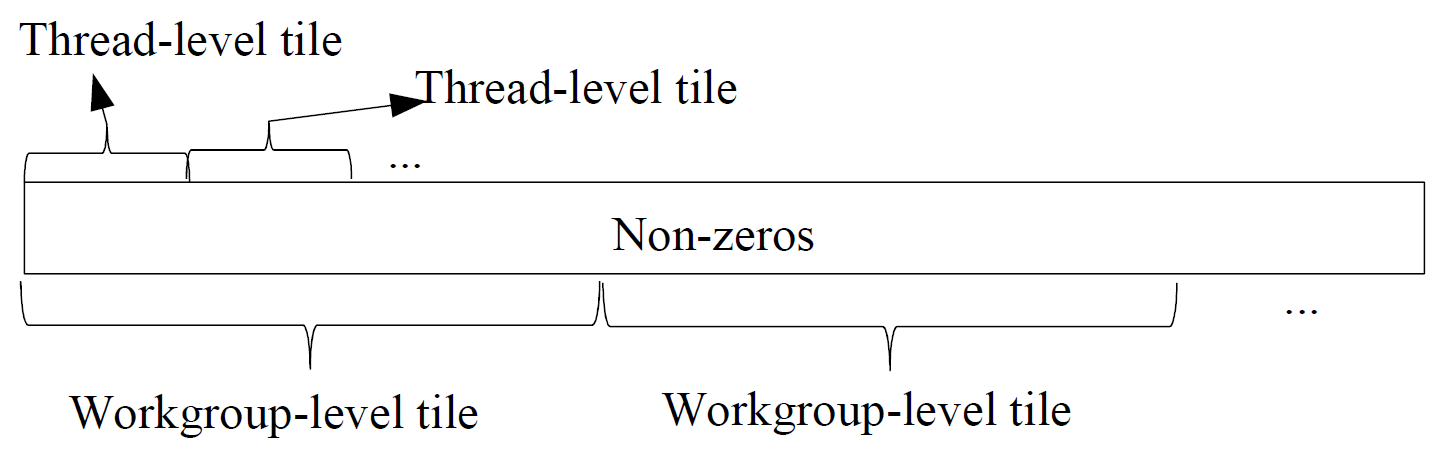
\includegraphics[scale=0.2]{figure/fig1-workload.png}
	\end{figure}
\end{frame}

\subsection{Matrix-based Segmented Sum/Scan}
\begin{frame}
	\frametitle{Matrix-based Strategy 1}
	\begin{itemize}
		\item Create \lstinline{intermediate_sums} in shared memory.
		\item If the lengths of segments are small, this strategy
			works well.
	\end{itemize}
\end{frame}
\begin{frame}
	\frametitle{Matrix-based Strategy 1 Example}
	\begin{figure}
		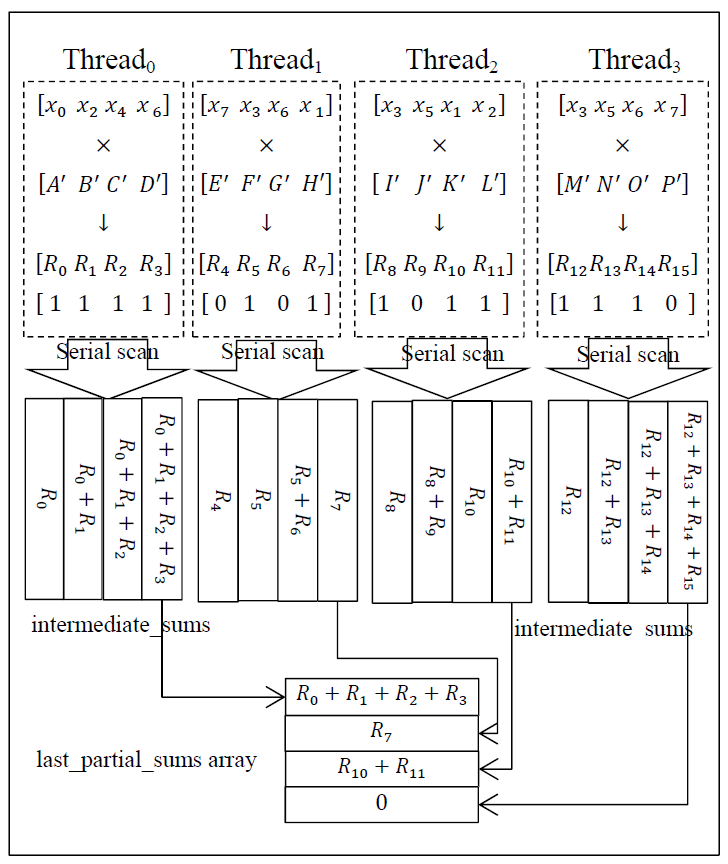
\includegraphics[scale=0.25]{figure/fig2-strategy1.png}
	\end{figure}
\end{frame}

\begin{frame}
	\frametitle{Matrix-based Strategy 2}
	\begin{itemize}
		\item Create result cache to store segmented sums.
		\item If the lenghts of segments are long, this strategy
			writes efficient-memory when we store result cache to
			global memory.
	\end{itemize}
\end{frame}
\begin{frame}
	\frametitle{Matrix-based Strategy 2 Example}
	\begin{figure}
		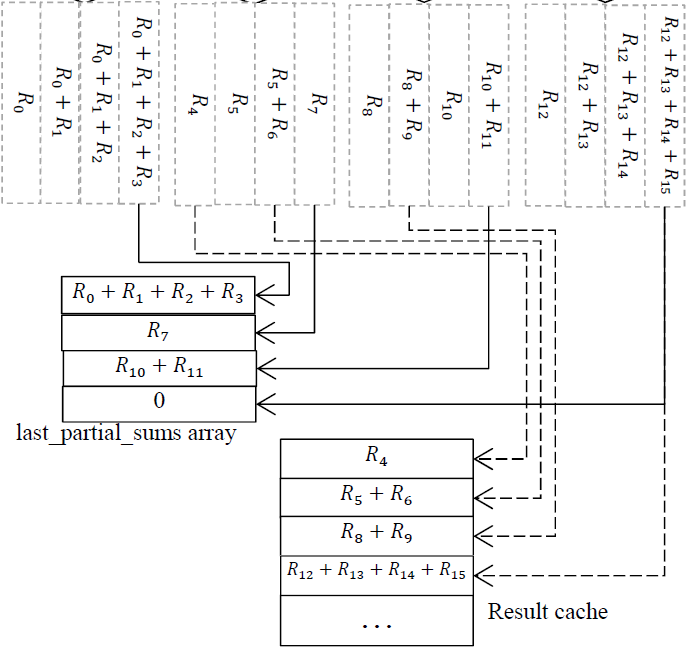
\includegraphics[scale=0.3]{figure/fig3-strategy2.png}
	\end{figure}
\end{frame}
\section{Auto-Tuning Framework}

\subsection{Auto-Tuning Framework}
\begin{frame}
	\frametitle{Auto-Tuning Framework}
	\begin{itemize}
		\item To find the optimal solution for a sparse matrix, build
			and auto-tuning framework to select the format.
	\end{itemize}
	\begin{figure}
		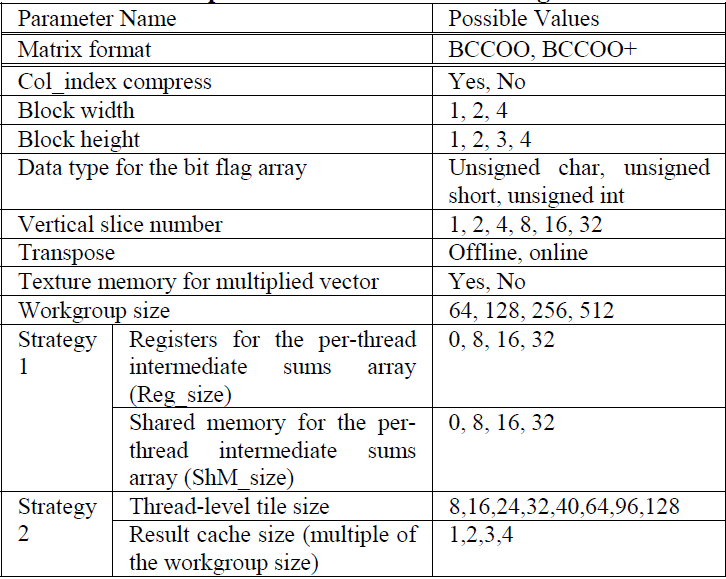
\includegraphics[scale=0.3]{figure/fig4-parameters.png}
	\end{figure}
\end{frame}
\section{Experiment}

\subsection{Sparse Matrices}
\begin{frame}
	\frametitle{Sparse Matrices}
	\begin{figure}
		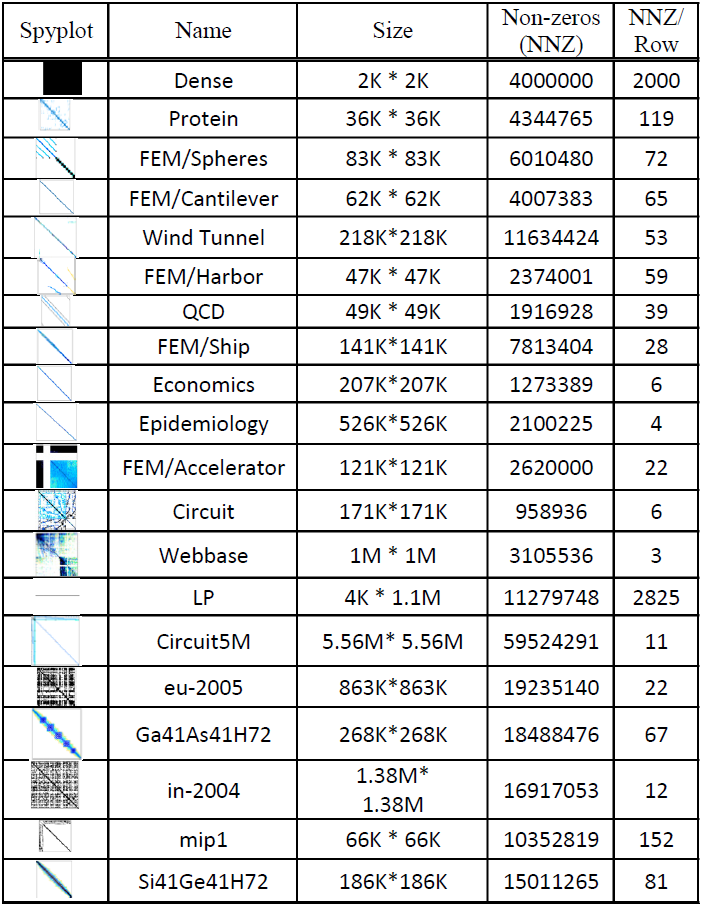
\includegraphics[scale=0.25]{figure/fig5-kindmatrices.png}
	\end{figure}
\end{frame}

\subsection{Memory Footprint}
\begin{frame}
	\frametitle{Memory Footprint}
	\begin{figure}
		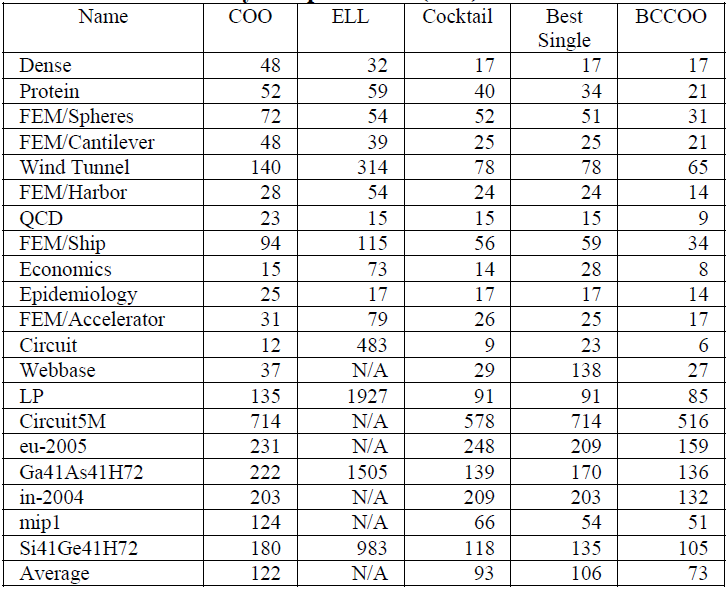
\includegraphics[scale=0.4]{figure/fig6-memoryprint.png}
	\end{figure}
\end{frame}

\subsection{Performance Comparison}
\begin{frame}
	\frametitle{Performance Comparison between Other Algorithms}
	\begin{figure}
		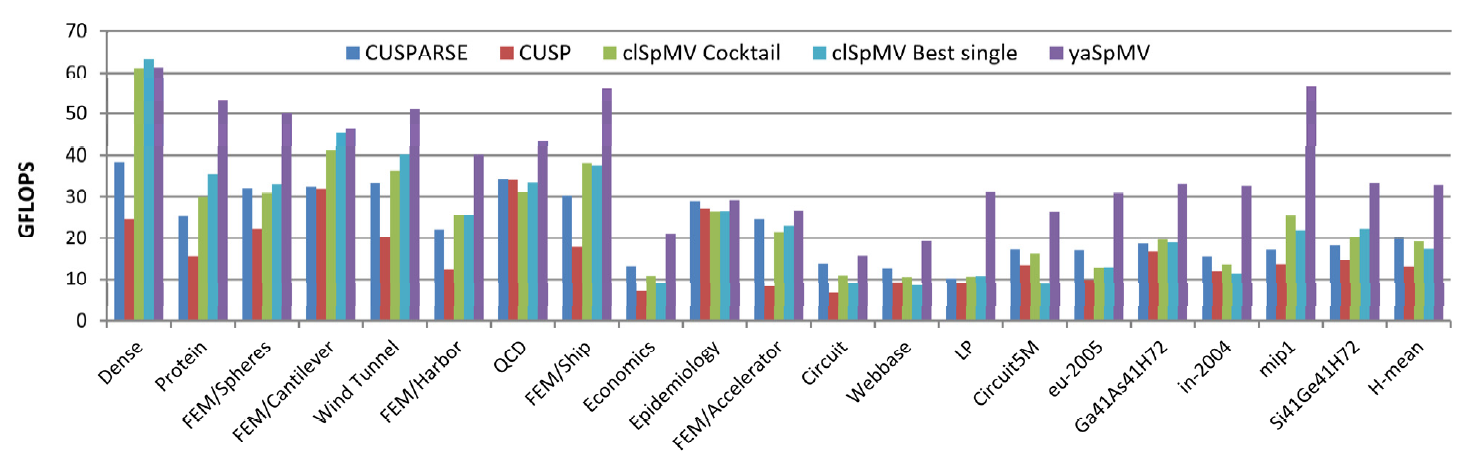
\includegraphics[scale=0.25]{figure/fig7-exp1.png}
	\end{figure}
\end{frame}

\begin{frame}
	\frametitle{Performance Comparison between Different Optimizations}
	\begin{figure}
		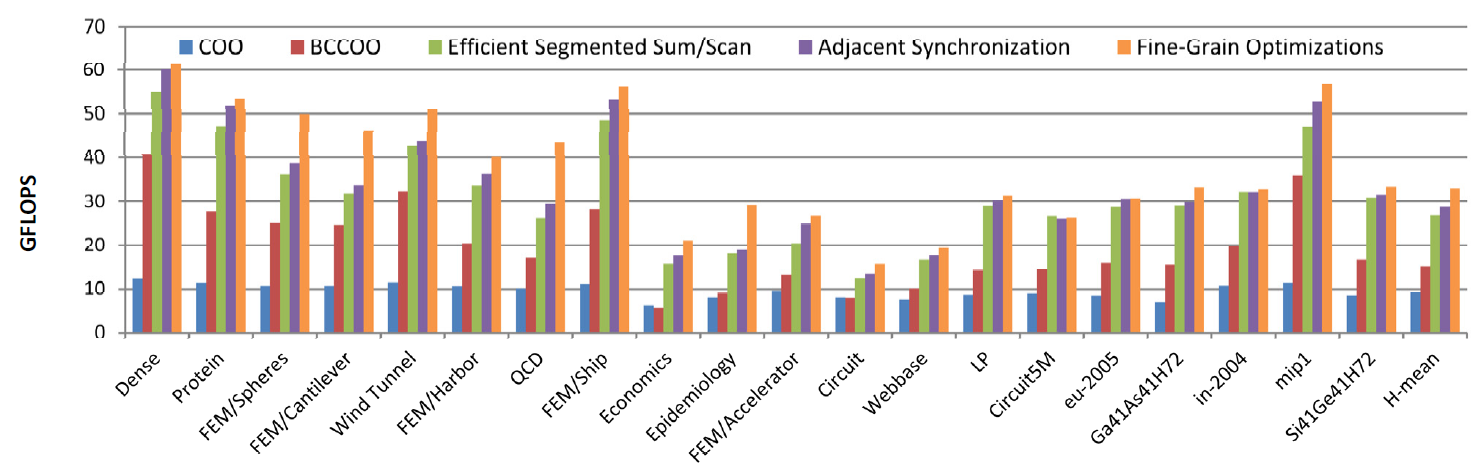
\includegraphics[scale=0.25]{figure/fig8-exp2.png}
	\end{figure}
\end{frame}
\section{Conclusions}

\subsection{Conclusions}
\begin{frame}
	\frametitle{Conclusions}
	\begin{itemize}
		\item This paper proposed new format: block compressed common coordinate
			(BCCOO) to improve locality for accesses to the multiplied vector.
		\item Combine Matrix-based segmented sum/scan and BCCOO/BCCOO+ format to
			reduce the memory bandwidth.
		\item It improves at least 40\% preformance.
	\end{itemize}
\end{frame}

\end{document}
